\section{Введение}

\begin{frame}[c]{Что такое NLP?}


\begin{itemize}
	\setbeamertemplate{itemize items}[square]
	\item NLP -- это способ  построения вычислительных алгоритмов для анализа, понимания и извлечения смысла с человеческого языка. 
\end{itemize}

\begin{figure}
\centering
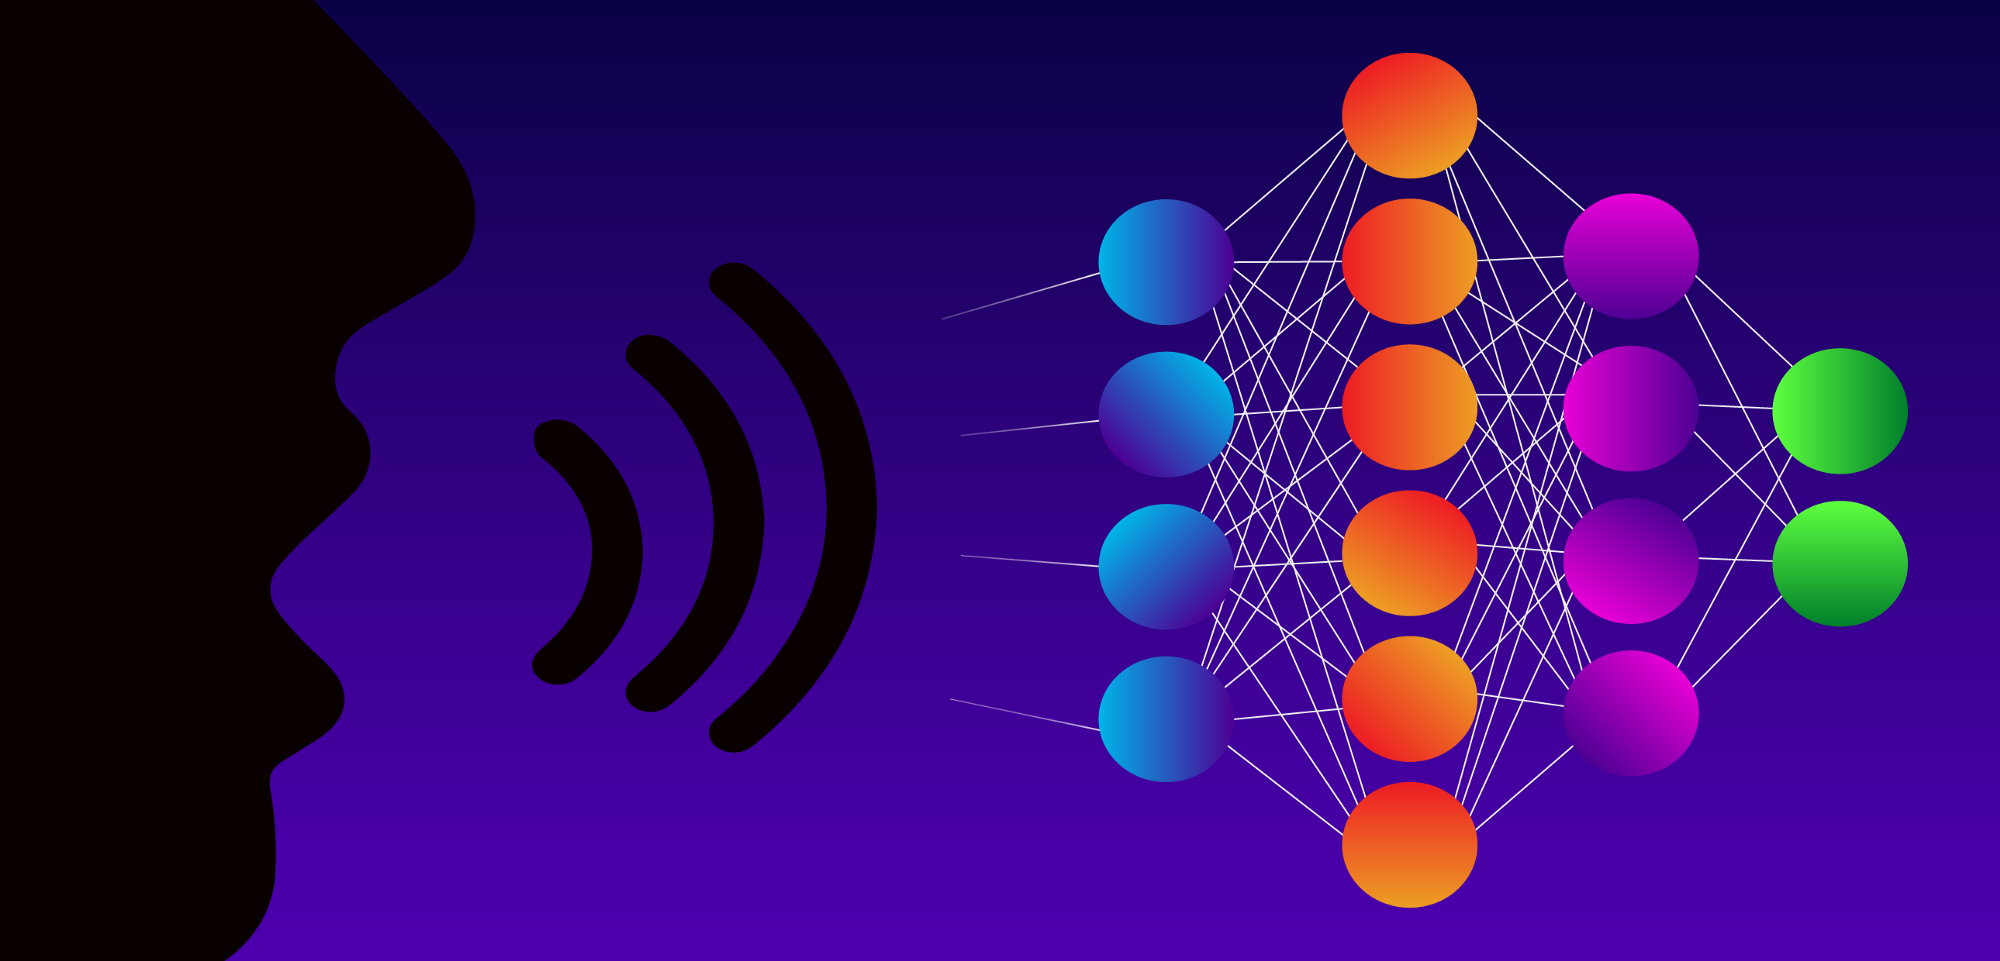
\includegraphics[width=0.8\textwidth]{figures/intro.png}
\end{figure}

\end{frame}

\begin{frame}[c]{Почему это сложно?}

\begin{itemize}
	\setbeamertemplate{itemize items}[square]
	\item Для понимания естественного языка нужно не просто правильным образом <<распарсить>> текст как последовательность букв или слов.
	\item Например, задача разрешение анафоры:
	\setbeamertemplate{itemize items}[circle]
	\begin{itemize}
		\item «Мама вымыла раму, и теперь она блестит».
		\item «Мама вымыла раму, и теперь она устала».
		\item К чему относится местоимение <<она>> в каждой из этих фраз?
	\end{itemize}
	\setbeamertemplate{itemize items}[square]
	\item Нужно иметь <<здравый смысл>>, представление об окружающем мире.
	
\end{itemize}
\end{frame}

\begin{frame}[c]{Примеры задач}

\begin{itemize}
	\setbeamertemplate{itemize items}[square]
	\item Задачи:
	\setbeamertemplate{itemize items}[circle]
	\begin{itemize}
		\item классификация текстов;
		\item тематическое моделирование;
		\item машинный перевод;
		\item автоматическое реферирование;
		\item диалоговые модели;
		\item ответы на вопросы;
		\item \dots
	\end{itemize}
	\setbeamertemplate{itemize items}[square]
	\item Сосредоточимся не на конкретных задачах, а на революции нейросетевых методов их решения.
\end{itemize}


\end{frame}